%Este trabalho está licenciado sob a Licença Creative Commons Atribuição-CompartilhaIgual 3.0 Não Adaptada. Para ver uma cópia desta licença, visite http://creativecommons.org/licenses/by-sa/3.0/ ou envie uma carta para Creative Commons, PO Box 1866, Mountain View, CA 94042, USA.

%\documentclass[main.tex]{subfiles}
%\begin{document}

\chapter{Derivação Numérica}\index{derivação}

Nesta seção, discutiremos sobre estratégias numéricas de aproximação de derivadas de funções reais. Com as técnicas que abordaremos é possível o cálculo aproximado da derivada de uma função a partir de um conjunto de pontos discretos $\{(x_i, y_i)\}_{i=1}^n$. Começamos discutindo sobre as chamadas \emph{aproximações por diferenças finitas}\index{aproximações por diferenças finitas} e, então, discutimos sobre aproximações de derivadas via ajuste ou interpolação.

%%%%%%%%%%%%%%%%%%%%
% python
%%%%%%%%%%%%%%%%%%%%
\ifispython
Ao longo deste capítulo, estaremos assumindo que as seguintes bibliotecas e módulos \verb+Python+ estão importados:
\begin{verbatim}
from __future__ import division
import numpy as np
import matplotlib.pyplot as plt
\end{verbatim}
\fi
%%%%%%%%%%%%%%%%%%%%

\section{Diferenças finitas}\index{diferenças finitas}

Uma diferença finita é uma expressão da forma $f(x+b)-f(x+a)$, que ao ser dividida por $(b-a)$ chama-se um quociente de diferenças. A técnica de \emph{diferenças finitas}\index{diferenças finitas} consiste em aproximar a derivada de uma função via fórmulas discretas que requerem apenas um conjunto finito de pares ordenados $\left\{\left(x_i, y_i\right)\right\}_{i=1}^n$, onde geralmente denotamos $y_i=f(x_i)$.

Essas fórmulas podem ser obtidas de várias maneiras. Começamos com a fórmula mais simples que pode ser obtida do cálculo diferencial. Seja $f$ uma função diferenciável, a derivada de $f$ no ponto $x_0$ é, por definição,
\begin{equation*}
  f'(x_0)=\lim_{h\to 0}\frac{f(x_0+h)-f(x_0)}{h}.
\end{equation*}
Deste limite, tomando $h\neq 0$ pequeno (não muito pequeno para evitar o cancelamento catastrófico), é esperado que possamos obter uma aproximação razoável para $f'(x_0)$. Assim, a \emph{diferença finita progressiva} de ordem 1
\begin{equation}\label{eq:dp}
  D_{+,h}f(x_0) := \frac{f(x_0+h)-f(x_0)}{h} \approx f'(x_0)
\end{equation}
é uma aproximação para $f'(x_0)$.

\begin{ex}\label{ex:dp}
Usando a diferença finita progressiva de ordem 1, calcule aproximações da derivada de $f(x)=\cos(x)$ no ponto $x=1$ usando $h=10^{-1}$, $10^{-2}$, $10^{-3}$, $10^{-4}$, $10^{-12}$ e $10^{-14}$. Calcule o erro $|D_{+,h}f(1)-f'(1)|$ obtido para cada valor de $h$.
\end{ex}
\begin{sol}
Usando a diferença progressiva em ~\eqref{eq:dp}, devemos calcular
\begin{equation*}
  D_{+,h}f(1) = \frac{\cos(1 + h) - \cos(1)}{h}
\end{equation*}
Fazendo isso, obtemos:
\begin{center}
  \begin{tabular}{r|c|c}
    $h$        & $D_{+,h}f(1)$   & $|f'(1) - D_{+,h}f(1)|$ \\ \hline
    $10^{-1}$  & $-8,67062\E-01$ & $2,55909\E-02$\\
    $10^{-2}$  & $-8,44158\E-01$ & $2,68746\E-03$\\
    $10^{-3}$  & $-8,41741\E-01$ & $2,70011\E-04$\\
    $10^{-4}$  & $-8,41498\E-01$ & $2,70137\E-05$ \\
    $10^{-12}$ & $-8,41549\E-01$ & $7,80679\E-05$\\
    $10^{-14}$ & $-8,43769\E-01$ & $2,29851\E-03$ \\\hline
  \end{tabular}
\end{center}

%%%%%%%%%%%%%%%%%%%%
% scilab
%%%%%%%%%%%%%%%%%%%%
\ifisscilab
No \verb+Scilab+, podemos calcular a aproximação da derivada $f'(1)$ com $h=0,1$ usando as seguintes linhas de código:
\begin{verbatim}
--> deff('y = f(x)','y = cos(x)')
--> x0 = 1
--> h  = 0.1
--> df = (f(x0+h) - f(x0))/h
\end{verbatim}
E, similarmente, para outros valores de $x_0$ e $h$.
\fi
%%%%%%%%%%%%%%%%%%%%
%%%%%%%%%%%%%%%%%%%%
% octave
%%%%%%%%%%%%%%%%%%%%
\ifisoctave
No \verb+GNU Octave+, podemos calcular a aproximação da derivada $f'(1)$ com $h=0,1$ usando as seguintes linhas de código:
\begin{verbatim}
f = @(x) cos(x);
x0 = 1;
h = 0.1;
df = (f(x0+h) - f(x0))/h
\end{verbatim}
E, similarmente, para outros valores de $x_0$ e $h$.
\fi
%%%%%%%%%%%%%%%%%%%%
%%%%%%%%%%%%%%%%%%%%
% python
%%%%%%%%%%%%%%%%%%%%
\ifispython
Em \verb+Python+, podemos calcular a aproximação da derivada $f'(1)$ com $h=0,1$ usando as seguintes linhas de código:
\begin{verbatim}
>>> def f(x):
...    return np.cos(x)
...
>>> x0=1
>>> h=0.1
>>> df = (f(x0+h)-f(x0))/h
\end{verbatim}
E, similarmente, para outros valores de $x_0$ e $h$.
\fi
%%%%%%%%%%%%%%%%%%%%
\end{sol}

\begin{figure}
  \centering
  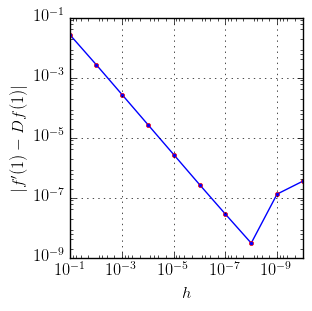
\includegraphics{./cap_derivacao/pics/ex_derivacao/ex_derivacao}
  \caption{Erro absoluto das derivadas numéricas no exemplo~\ref{ex:dp}.}
  \label{fig:ex_derivacao}
\end{figure}

Exploremos o exemplo~\ref{ex:dp} um pouco mais. Observamos que, para valores moderados de $h$, o erro $|f'(1)-D_{+,h}f(1)|$ diminui linearmente com $h$ (veja figura~\ref{fig:ex_derivacao}). Isto é consequência da ordem de truncamento da fórmula de diferenças finitas aplicada (que é de ordem 1). Porém, para valores muito pequenos de $h < 10^{-8}$, o erro passa a aumentar quando diminuímos $h$. Isto é devido ao efeito de cancelamento catastrófico.

\subsection{Diferenças finitas via série de Taylor}

Podemos construir fórmulas de diferenças finitas para uma função $f(x)$ (suave\footnote{Uma função suave é uma função infinitamente continuamente diferenciável, isto é, $f\in C^\infty(\mathbb{R})$. Uma análise mais cuidadosa, revela que hipóteses mais fracas podem ser assumidas.}) no ponto $x = x_0$ a partir de sua expansão em série de Taylor. Em alguns casos, este procedimento acaba por nos fornecer, também, a ordem de truncamento da fórmula.

\subsubsection{Diferença finita progressiva de ordem 1}\index{diferenças finitas!progressiva}
Podemos obter uma aproximação para $f'(x_0)$ a partir da série de Taylor
\begin{equation*}
  f(x_0+h) = f(x_0) + hf'(x_0) + h^2\frac{f''(\xi)}{2},\quad h>0, \xi\in(x_0,x_0+h).
\end{equation*}
Isolando $f'(x_0)$, obtemos
\begin{equation}\label{eq:dp_trunc}
  f'(x_0) = \underbrace{\frac{f(x_0+h) - f(x_0)}{h}}_{D_{+,h}} - \underbrace{h\frac{f''(\xi)}{2}}_{\mathcal{O}(h)},
\end{equation}
o que mostra que o erro de truncamento da \emph{diferença finita progressiva}\footnote{Também chamada de diferença finita progressiva de dois pontos ou diferença pra frente.}
\begin{equation*}
  D_{+,h}f(x_0) := \frac{f(x_0+h)-f(x_0)}{h}
\end{equation*}
é de ordem $h$.

\subsubsection{Diferença finita regressiva de ordem 1}\index{diferenças finitas!regressiva}
Outra aproximação para a derivada primeira pode ser obtida da série de Taylor de $f$ em torno de $(x_0-h)$ dada por
\begin{equation*}
  f(x_0-h) = f(x_0) - hf'(x_0) + h^2\frac{f''(\xi)}{2},\quad h>0, \xi\in(x_0, x_0+h).
\end{equation*}
Isolando $f'(x_0)$, obtemos
\begin{equation*}
  f'(x_0) = \underbrace{\frac{f(x_0) - f(x_0-h)}{h}}_{D_{-,h}} + \underbrace{h\frac{f''(\xi)}{2}}_{\mathcal{O}(h)}.
\end{equation*}
que fornece a \emph{diferença finita regressiva}\footnote{Também chamada de diferença regressiva de dois pontos ou diferença pra trás.}
\begin{equation*}
  D_{-,h}f(x_0) := \frac{f(x_0)-f(x_0-h)}{h},
\end{equation*}
que possui erro de truncamento de ordem $h$.

\subsubsection{Diferença finita central de ordem 2}\index{diferenças finitas!central}
Para obter uma aproximação para a derivada primeira com um erro menor, podemos utilizar as séries de Taylor:
\begin{eqnarray*}
    f(x_0+h) &= f(x_0) + hf'(x_0) + h^2f''(x_0) + h^3\frac{f'''(\xi_{+})}{3!},\\
    f(x_0-h) &= f(x_0) - hf'(x_0) + h^2f''(x_0) + h^3\frac{f'''(\xi_{-})}{3!}
\end{eqnarray*}
Fazendo a primeira equação menos a segunda, obtemos
\begin{equation*}
  f(x_0+h)-f(x_0-h) = 2hf'(x_0) + h^{3}\left(\frac{f'''(\xi_{+}) - f'''(\xi_{-})}{3!}\right).
\end{equation*}
Dividindo por $2h$ e isolando $f'(x_0)$ obtemos
\begin{equation*}
  f'(x_0) = \underbrace{\frac{f(x_0+h) - f(x_0-h)}{2h}}_{D_{0,h}} - \underbrace{h^2\left(\frac{f'''(\xi_+) - f'''(\xi_-)}{2\cdot 3!}\right)}_{\mathcal{O}(h^2)}.
\end{equation*}
Assim, a \emph{diferença finita central}\footnote{Também chamada de diferença finita central de três pontos. Note que o ponto $f(x_0)$ possui coeficiente $0$, por isso $3$ pontos.}
\begin{equation*}
  D_{0,h}f(x_0) := \frac{f(x_0+h)-f(x_0-h)}{2h},
\end{equation*}
é uma aproximação para $f'(x_0)$ com erro de truncamento de ordem $h^2$, ou simplesmente ordem $2$.

\begin{ex}\label{ex:derivacao2}
Calcule a derivada numérica da função $f(x)=e^{\frac{1}{2}x}$ no ponto $x=2$ usando a diferença progressiva, diferença regressiva e diferença central com $h=10^{-1}$, $h=10^{-2}$ e $h=10^{-4}$. Também, calcule o erro absoluto da aproximação obtida em cada caso.
\end{ex}
\begin{sol}
  Usando a diferença progressiva, devemos calcular
  \begin{equation*}
    D_{+,h} = \frac{f(x+h) - f(x)}{h} = \frac{e^{\frac{1}{2}(x+h)} - e^{\frac{1}{2}x}}{h}.
  \end{equation*}
  Com a diferença regressiva, calculamos
  \begin{equation*}
    D_{-,h} = \frac{f(x) - f(x-h)}{h} = \frac{e^{\frac{1}{2}x} - e^{\frac{1}{2}(x-h)}}{h}.
  \end{equation*}
  Por fim, usando a diferença central temos
  \begin{equation*}
    D_{0,h} = \frac{f(x+h) - f(x-h)}{2h} = \frac{e^{\frac{1}{2}(h+h)} - e^{\frac{1}{2}(x-h)}}{2h}.
  \end{equation*}

  As aproximações e os erros absolutos calculados em cada caso estão apresentados na seguinte tabela:
  \begin{center}
    \begin{tabular}{r|cc|cc|cc}
      $h$  & $D_{+,h}f(2)$ & Erro & $D_{-,h}$ & Erro & $D_{0,h}$ & Erro \\\hline
      $10^{-1}$ & $1,39369$ & $3,5\E-02$   & $1,32572$ & $3,3\E-02$ & $1,35971$ & $5,7\E-04$\\
      $10^{-2}$ & $1,36254$ & $3,4\E-03$   & $1,35575$ & $3,4\E-03$ & $1,35915$ & $5,7\E-06$\\
      $10^{-4}$ & $1,35917$ & $3,4\E-05$   & $1,35911$ & $3,4\E-05$ & $1,35914$ & $5,7\E-10$\\\hline
    \end{tabular}
  \end{center}
\end{sol}

\begin{figure}
  \centering
  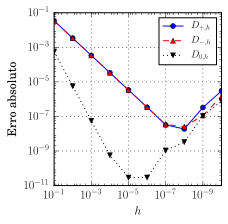
\includegraphics{./cap_derivacao/pics/ex_derivacao2/ex_derivacao2}
  \caption{Erro absoluto das derivadas numéricas no exemplo~\ref{ex:derivacao2}.}
  \label{fig:ex_derivacao2}
\end{figure}


\begin{obs}
  O experimento numérico realizado no exemplo~\ref{ex:derivacao2}, nos mostra que o erro absoluto na derivação numérica não é da ordem do erro de truncamento. Entretanto, este erro tende a variar com $h$ na mesma ordem do erro de truncamento. A figura~\ref{ex:derivacao2} apresenta o erro absoluto das derivadas numéricas computadas para o exemplo~\ref{ex:derivacao2}. Note que, devido ao efeito de cancelamento catastrófico, o erro absoluto deixa de variar na ordem do erro de truncamento para valores muito pequenos de $h$.
\end{obs}

% \subsection{Erros de truncamento}\index{erros!truncamento}
% Seja $D_{+,h}f(x_0)$ a aproximação da derivada de $f$ em $x_0$ por diferenças progressivas, $D_{-,h}f(x_0)$ a aproximação por diferenças regressivas e $D_{0,h}f(x_0)$ a aproximação por diferenças centrais, então
% \begin{eqnarray*}
% D_{+,h}f(x_0)-f'(x_0)&=&\frac{f(x_0+h)-f(x_0)}{h}-f'(x_0)\\
% &=&\frac{f(x_0)+hf'(x_0)+\frac{h^2}{2}f''(x_0)+\mathcal{O}(h^3)-f(x_0)}{h}-f'(x_0)\\
% &=&\frac{h}{2}f''(x_0)+\mathcal{O}(h^2)=\mathcal{O}(h).\\
% \end{eqnarray*}
% Analogamente:
% \begin{eqnarray*}
% D_{-,h}f(x_0)-f'(x_0)&=&\frac{f(x_0)-f(x_0-h)}{h}-f'(x_0)\\
% &=&\frac{f(x_0)-\left(f(x_0)-hf'(x_0)+\frac{h^2}{2}f''(x_0)+\mathcal{O}(h^3)\right)}{h}-f'(x_0)\\
% &=&-\frac{h}{2}f''(x_0)+\mathcal{O}(h^2)=\mathcal{O}(h).\\
% \end{eqnarray*}
% Também:
% \begin{eqnarray*}
% D_{0,h}f(x_0)-f'(x_0)&=& \frac{f(x_0+h)-f(x_0-h)}{2h}-f'(x_0)\\
% &=& \frac{f(x_0)+hf'(x_0)+\frac{h^2}{2}f''(x_0)+\mathcal{O}(h^3)}{2h} \\
% &-& \frac{f(x_0)-hf'(x_0)+\frac{h^2}{2}f''(x_0)+\mathcal{O}(h^3)}{2h}-f'(x_0)\\
% &=& \mathcal{O}(h^2).
% \end{eqnarray*}

\begin{ex}
Estime o erro absoluto no cálculo da derivada de $f(x)=e^{-x}$ para $x>0$ utilizando a diferença progressiva.
\end{ex}
\begin{sol}
Da equação~\ref{eq:dp_trunc}, temos:
\begin{equation*}
  f'(x) = D_{+,h}f(x) - h\frac{f''(\xi)}{2},\quad \xi>0,
\end{equation*}
ou seja:
\begin{equation*}
  |f'(x) - D_{+,h}f(x)| = \left|\frac{f''(\xi)}{2}\right|h,\quad \xi>0.
\end{equation*}
Agora, como $|f''(x)| = |e^{-x}| < 1$ para $x>0$, concluímos que:
\begin{equation*}
  |f'(x) - D_{+,h}f(x)| \leq \frac{1}{2}h,\quad x>0.
\end{equation*}
\end{sol}

\subsection{Erros de arredondamento}\index{erros!arredondamento}
Para entender como os erros de arredondamento se propagam ao calcular as derivadas numéricas vamos analisar a fórmula de diferenças finitas progressiva
\begin{equation*}
  D_{+,h}f(x) =\frac{f(x+h)-f(x)}{h}.  
\end{equation*}

Nesse contexto temos o valor exato $f'(x)$ para a derivada, a sua aproximação numérica $D_{+,h}f(x)$ e a representação em número de máquina do operador $D_{+,h}f(x)$ que denotaremos por $\overline{D_{+,h}f(x)}$. Denotando por $\varepsilon(x,h)$ o erro de arredondamento ao calcularmos a derivada, vamos assumimos que
\begin{equation}\label{ex:ea_dp}
\overline{D_{+,h}f(x)}=D_{+,h}f(x)(1+\varepsilon(x,h))=\frac{\overline{f(x+h)}-\overline{f(x)}}{h}(1+\varepsilon(x,h)).  
\end{equation}
Também, consideremos
\begin{equation*}
|\overline{f(x+h)}-f(x+h)|=\delta(x,h)\leq \delta  
\end{equation*}
e
\begin{equation*}
  |\overline{f(x)}-f(x)|=\delta(x,0)\leq \delta,  
\end{equation*}
onde $\overline{f(x+h)}$ e $\overline{f(x)}$ são as representações em ponto flutuante dos números $f(x+h)$ e $f(x)$, respectivamente. 

Então, da equação~\eqref{ex:ea_dp}, a diferença do valor da derivada e sua aproximação representada em ponto flutuante pode ser estimada por:
\begin{equation*}
\left|f'(x)-\overline{D_{+,h}f(x)}\right| = \left| f'(x)-\frac{\overline{f(x+h)}-\overline{f(x)}}{h}(1+\varepsilon(x,h)) \right|.
\end{equation*}
Podemos reescrever o lado direito desta equação, da seguinte forma
\begin{eqnarray*}
  \left|f'(x)-\overline{D_{+,h}f(x)}\right| &=& \left| f'(x)-\left(\frac{\overline{f(x+h)}-\overline{f(x)}}{h}+\frac{f(x+h)-f(x+h)}{h}\right.\right. \\
&+& \left.\left.\frac{f(x)-f(x)}{h}\right)(1+\varepsilon) \right|\\
&=& \left| f'(x)+\left(-\frac{f(x+h)-f(x)}{h}-\frac{\overline{f(x+h)}-f(x+h)}{h}\right.\right.\\
&+& \left.\left. \frac{\overline{f(x)}-f(x)}{h}\right)(1+\varepsilon) \right|.
\end{eqnarray*}
Então, separando os termos e estimando, obtemos:
\begin{eqnarray*}
\left|f'(x)-\overline{D_{+,h}f(x)}\right| &\leq& \left|f'(x)-\frac{f(x+h)-f(x)}{h}\right| +\left(\left|\frac{\overline{f(x+h)}-f(x+h)}{h}\right|\right.\\
&+&\left.\left|\frac{\overline{f(x)}-f(x)}{h}\right| \right)|1+\varepsilon| + \left|\frac{f(x+h)-f(x)}{h}\right|\varepsilon\\
&\leq& Mh +\left(\left|\frac{\delta}{h}\right|+\left|\frac{\delta}{h}\right| \right)|1+\varepsilon| +|f'(x)|\varepsilon\\
&\leq& Mh +\left(\frac{2\delta}{h}\right)|1+\varepsilon| +|f'(x)|\varepsilon
\end{eqnarray*}
onde
$$
M=\frac{1}{2}\max_{x\leq y\leq x+h}|f''(y)|
$$
está relacionado com o erro de truncamento.

Por fim, obtemos a seguinte estimativa para o erro absoluto na computação da derivada numérica:
\begin{equation}\label{eq:est_erro_arredondamento}
  \left|f'(x)-\overline{D_{+,h}f(x)}\right| \leq Mh +\left(\frac{2\delta}{h}\right)|1+\varepsilon| +|f'(x)|\varepsilon.
\end{equation}

Esta estimativa mostra que se o valor de $h$ for muito pequeno o erro ao calcular a aproximação numérica cresce. Isso nos motiva a procurar o valor ótimo de $h$ que minimiza o erro.

\begin{ex}
No exemplo~\ref{ex:derivacao2}, computamos a derivada numérica da função $f(x)=e^{\frac{1}{2}x}$ no ponto $x=2$ usando as fórmulas de diferenças finitas progressivas, regressivas e central. A figura~\ref{fig:ex_derivacao2}, mostra que, para valores $h$ muito pequenos, os erros de arredondamento passam a dominar os cálculos e, por consequência, o erro da derivada numérica passa a aumentar. Pela figura, podemos inferir que a escolha ótima de $h$ para as fórmulas progressiva e regressivas é $h\approx 10^{-7}$. Agora, para a fórmula central, $h\approx 10^{-5}$ parece ser a melhor escolha.
\end{ex}

\begin{obs}
  Note que a estimativa~\eqref{eq:est_erro_arredondamento}, mostra que o erro na computação da derivada numérica depende da função que está sendo derivada. Assim, o $h$ ótimo depende não somente da fórmula de diferenças finitas, mas também da função a ser derivada.
\end{obs}

\subsection*{Exercícios Resolvidos}

\begin{exeresol}
Aproxime a derivada de $f(x)=\sen(2x) - x^2$ no ponto $x=2$ usando a fórmula de diferenças finitas progressiva de ordem 1 com: a) $h=0,1$ e b) $h=0,01$. Compute, também, o erro absoluto de cada aproximação computada.
\end{exeresol}
\begin{resol}
  A fórmula de diferenças finitas de ordem 1 para uma função $y = f(x)$ em um ponto $x = x_0$ é dada por:
  \begin{equation*}
    D_{+,h}f(x_0) = \frac{f(x_0+h) - f(x_0)}{h}.
  \end{equation*}
Substituindo $f(x) = \sen(2x) - x^2$ e $x_0 = 2$, obtemos:
  \begin{equation*}
    \begin{split}
      D_{+,h}f(x_0) &= \frac{(\sen(2(x_0+h)) - (x_0+h)^2) - (\sen(2x_0) - x_0^2)}{h}\\
      &= \frac{\sen(2(x_0+h)) - x_0^2 + 2x_0h + h^2 - \sen(2x_0) + x_0^2)}{h}\\
      &= \frac{\sen(4+2h) + 4h + h^2 - \sen(4))}{h}.
    \end{split}
  \end{equation*}
Então, tomando $h=0,1$, podemos computar a derivada numérica e o erro associado:
\begin{equation*}
  D_{+,0,1}f(2) = -5,247733,\quad |f'(2)-D_{+,0,1}f(2)| = 5,96\times 10^{-2},
\end{equation*}
onde $f'(x) = 2\sen(2x) - 2x$ é a derivada analítica. Tomando $h=0,01$ temos:
\begin{equation*}
  D_{+,0,1}f(2) = -5,302065,\quad |f'(2)-D_{+,0,1}f(2)| = 5,22\times 10^{-3}.
\end{equation*}

%%%%%%%%%%%%%%%%%%%%
% GNU octave
%%%%%%%%%%%%%%%%%%%%
\ifisoctave
No \verb+GNU Octave+, podemos fazer os cálculos com o seguinte código:
\begin{verbatim}
#funcao
f = @(x) sin(2*x) - x^2;

#derivada analitica
fl = @(x) 2*cos(2*x) - 2*x;

#d.f. progressiva de ordem 1
dp1 = @(f,x,h=0.1) (f(x+h)-f(x))/h;

#h=0.1
dy = dp1(f,2)
printf("D.F. Progressiva de ordem 1 com h = %f\n", 1e-1)
printf("Df = %f\n", dy)
printf("Erro = %1.2e\n", abs(fl(2)-dy))

#h=0.01
dy = dp1(f,2,1e-2)
printf("D.F. Progressiva de ordem 1 com h = %f\n", 1e-2)
printf("Df = %f\n", dy)
printf("Erro = %1.2e\n", abs(fl(2)-dy))
\end{verbatim}
\fi
%%%%%%%%%%%%%%%%%%%%
%%%%%%%%%%%%%%%%%%%%
% python
%%%%%%%%%%%%%%%%%%%%
\ifispython
Em \verb+Python+, podemos fazer os cálculos com o seguinte código:
\begin{verbatim}
#funcao
def f(x):
    return np.sin(2*x) - x**2

#derivada analitica
def fl(x):
    return 2*np.cos(2*x) - 2*x

#d.f. progressiva de ordem 1
def dp1(f,x,h=0.1):
    return (f(x+h)-f(x))/h

#h=0.1
dy = dp1(f,2)
print("D.F. Progressiva de ordem 1 com h = %f" % 1e-1)
print("Df = %f" % dy)
print("Erro = %1.2e" % np.abs(fl(2)-dy))

#h=0.01
dy = dp1(f,2,1e-2)
print("D.F. Progressiva de ordem 1 com h = %f" % 1e-2)
print("Df = %f" % dy)
print("Erro = %1.2e" % np.abs(fl(2)-dy))
\end{verbatim}
\fi
%%%%%%%%%%%%%%%%%%%%
\end{resol}


\subsection*{Exercícios}

\begin{exer}
Use os esquemas numéricos do exercício \ref{ex1} para aproximar as seguintes derivadas:
\begin{itemize}
\item[a)] $f'(x)$ onde $f(x)=\sen(x)$ e $x=2$.
\item[b)] $f'(x)$ onde $f(x)=e^{-x}$ e $x=1$.
\end{itemize}
Use $h=10^{-2}$ e $h=10^{-3}$ e compare com os valores obtidos através da avaliação numérica das derivadas exatas.
\end{exer}

\begin{exer}\label{ex1} Expanda a função suave $f(x)$ em um polinômio de Taylor adequado para obter as seguintes aproximações:
\begin{itemize}
\item[a)] $f'(x)=\frac{f(x+h)-f(x)}{h}+\mathcal{O}(h)$
\item[b)] $f'(x)=\frac{f(x)-f(x-h)}{h}+\mathcal{O}(h)$
\item[c)] $f'(x)=\frac{f(x+h)-f(x-h)}{2h}+\mathcal{O}(h^2)$
\end{itemize}
\end{exer}


\begin{exer} Use a expansão da função $f(x)$ em torno de $x=0$ em polinômios de Taylor para encontrar os coeficientes $a_1$, $a_2$ e $a_3$ tais que
\begin{itemize}
\item[a)] $f'(0)=a_1f(0)+a_2f(h)+a_3f(2h) + \mathcal{O}(h^2)$
\item[b)] $f'(0)=a_1f(0)+a_2f(-h)+a_3f(-2h) + \mathcal{O}(h^2)$
\item[c)] $f'(0)=a_1f(-h_1)+a_2f(0)+a_3f(h_2) + \mathcal{O}(h^2),~~|h_1|, |h_2|=\mathcal{O}(h)$
\end{itemize}
\end{exer}
\begin{resp}
%  
\begin{itemize}
\item[a)] $f'(0)=\frac{-3f(0)+4f(h)-f(2h)}{2h} + \mathcal{O}(h^2)$
\item[b)] $f'(0)=\frac{3f(0)-4f(-h)+f(-2h)}{2h} + \mathcal{O}(h^2)$
\item[c)] $f'(0)=\frac{1}{h_1+h_2}l\left[-\frac{h_2}{h_1}f(-h_1) +\left(\frac{h_2}{h_1}-\frac{h_1}{h_2}\right)f(0)+ \frac{h_1}{h_2}f(h_2)\right]$
\end{itemize}    
%  
\end{resp}

\begin{exer} As tensões  na entrada, $v_i$, e saída, $v_o$, de um amplificador foram medidas em regime estacionário conforme tabela abaixo.
  \begin{center}
    \begin{tabular}{|c|c|c|c|c|c|c|c|c|c|c|}\hline
    0,0 &   0,50  &   1,00   &   1,50  &   2,00 &     2,50   &  3,00  &    3,50  &   4,00  &    4,50  &   5,00\\ \hline
    0,0  &  1,05  &  1,83  &  2,69  &  3,83 &   4,56 &   5,49 &   6,56  &  6,11 &   7,06  &  8,29\\ \hline 
    \end{tabular}
  \end{center}
onde  a primeira linha é a tensão de entrada em volts e a segunda linha é tensão de saída em volts.
Sabendo que o ganho é definido como $$\frac{\partial v_o}{\partial v_i}.$$ Calcule o ganho quando $v_i=1$ e $v_i=4.5$ usando as seguintes técnicas:
\begin{itemize}
\item[a)] Derivada primeira numérica de primeira ordem usando o próprio ponto e o próximo.
\item[b)] Derivada primeira numérica de primeira ordem usando o próprio ponto e o anterior.
\item[c)] Derivada primeira numérica de segunda ordem usando o ponto anterior e o próximo.
\item[d)] Derivada primeira analítica da função do tipo $v_0=a_1 v_i + a_3 v_i^3$ que melhor se ajusta aos pontos pelo critério dos mínimos quadrados.
\end{itemize}
\begin{center}
\begin{tabular}{|c|c|c|c|c|}\hline
 Caso &  a  &   b &   c   &   d \\ \hline
 $v_i=1$ &    & ~\hspace{50pt}~  &   & ~\hspace{50pt}~ \\ \hline
$v_i=4.5$ &~\hspace{50pt}~    &   &  ~\hspace{50pt}~   &\\ \hline
\end{tabular}
\end{center}
% \ifisscilab
% Dica:
% \begin{verbatim}
% y=[0 1.05 1.83 2.69 3.83 4.56 5.49 6.56 6.11 7.06 8.29]
% \end{verbatim}
% \fi
\end{exer}
\begin{resp}
$$\begin{array}{|c|c|c|c|c|}\hline
 Caso &  a  &   b &   c   &   d \\ \hline
 v_i=1 & 1.72   & 1.56  &  1.64 & 1.86 \\ \hline
v_i=4.5 &2.46    & 1.90  &  2.18  &1.14  \\ \hline
\multicolumn{5}{c}{}
\end{array}
$$    
\end{resp}

\begin{exer}Estude o comportamento da derivada de $f(x)=e^{-x^2}$ no ponto $x=1,5$ quando $h$ fica pequeno.
\end{exer}
\begin{resp}
  
Segue a tabela com os valores da derivada para vários valores de $h$.

\begin{equation*}
\begin{array}{|c|c|c|c|c|c|c|}\hline
h&10^{-2}&10^{-4}&10^{-6}&10^{-7}&10^{-8}&10^{-9}\\\hline
D_{+,h}f(1,5)& - 0,3125246&- 0,3161608 &- 0,3161973&- 0,3161976&- 0,3161977&- 0,3161977 \\\hline
\multicolumn{7}{c}{}
\end{array}  
\end{equation*}  
\begin{equation*}
\begin{array}{|c|c|c|c|c|c|c|}\hline
h&10^{-10}&10^{-11}&10^{-12}&10^{-13}&10^{-14}&10^{-15}\\\hline
D_{+,h}f(1,5)&- 0,3161976&- 0,3161971&- 0,3162332&- 0,3158585&- 0,3178013&- 0,3747003\\\hline
\multicolumn{7}{c}{}
\end{array}
\end{equation*}
Observe que o valor exato é $-0,3161977$ e o $h$ ótimo é algo entre $10^{-8}$ e $10^{-9}$.        
\end{resp}

\section{Diferença finita para derivada segunda}\index{fórmula de diferenças finitas!central}

Para aproximar a derivada segunda, considere as expansões em série de Taylor
$$
f(x_0+h)=f(x_0)+hf'(x_0)+\frac{h^2}{2}f''(x_0)+\frac{h^3}{6}f'''(x_0)+O(h^4)
$$
$$
f(x_0-h)=f(x_0)-hf'(x_0)+\frac{h^2}{2}f''(x_0)-\frac{h^3}{6}f'''(x_0)+O(h^4).
$$
Somando as duas expressões, temos:
$$
f(x_0+h)+f(x_0-h)=2f(x_0)+h^2f''(x_0)+O(h^4)
$$
ou seja, uma aproximação de segunda ordem para a derivada segunda em $x_0$ é
$$
f''(x_0)=\frac{f(x_0+h)-2f(x_0)+f(x_0-h)}{h^2}+\mathcal{O}(h^2):=D^2_{0,h}f(x_0)+\mathcal{O}(h^2),
$$
onde
$$
D^2_{0,h}f(x_0)=\frac{f(x_0+h)-2f(x_0)+f(x_0-h)}{h^2}.
$$

\begin{ex}
Calcule a derivada segunda numérica de $f(x)=e^{-x^2}$ em $x=1,5$ para $h=0,1$, $h=0,01$ e $h=0,001$.
\end{ex}
\begin{sol}
A tabela mostra os resultados:
\begin{center}
  \begin{tabular}{|c|c|c|c|}\hline
    $h$ & $h=0,1$ & $h=0,01$ & $h=0,001$\\\hline
    $D^2_{0,h}f(1,5)$ & $0,7364712$ & $0,7377814$ & $0,7377944$\\\hline
  \end{tabular}  
\end{center}
Observe que $f''(x)=(4x^2-2)e^{-x^2}$ e $f''(1,5)=0,7377946$.  

%%%%%%%%%%%%%%%%%%%%
% GNU octave
%%%%%%%%%%%%%%%%%%%%
\ifisoctave
No \verb+GNU Octave+, podemos fazer os cálculos acima com o seguinte código:
\begin{verbatim}
#funcao
f = @(x) exp(-x^2);

#d.f. central para segunda derivada
d2c = @(f,x,h) (f(x-h)-2*f(x)+f(x+h))/(h^2);

x0 = 1.5;
d2c(f,x0,1e-1) #h=0.1
d2c(f,x0,1e-2) #h=0.01
d2c(f,x0,1e-3) #h=0.001
\end{verbatim}
\fi
%%%%%%%%%%%%%%%%%%%%
\end{sol}

\subsection*{Exercícios}

\begin{exer} Use a expansão da função $f(x)$ em torno de $x=0$ em polinômios de Taylor para encontrar os coeficientes $a_1$, $a_2$ e $a_3$ tais que
\begin{itemize}
\item[a)] $f''(0)=a_1f(0)+a_2f(h)+a_3f(2h) + \mathcal{O}(h)$
\item[b)] $f''(0)=a_1f(0)+a_2f(-h)+a_3f(-2h) + \mathcal{O}(h)$
\end{itemize}
\end{exer}
\begin{resp}
\begin{itemize}
\item[a)] $f''(0)=\frac{f(0)-2f(h)+f(2h)}{h^2}+\mathcal{O}(h)$
\item[b)] $f''(0)=\frac{f(0)-2f(-h)+f(-2h)}{h^2}+\mathcal{O}(h)$
\end{itemize}    
\end{resp}

\section{Obtenção de fórmulas por polinômios interpoladores}\index{diferenças finitas!ordem mais alta}

Para aproximar a derivada de uma função $f(x)$ em $x_0$, $x_1$ ou $x_2$ usaremos os três pontos vizinhos $(x_0,f(x_0))$, $(x_{1},f(x_{1}))$ e $(x_{2},f(x_{2}))$. Uma interpolação usando polinômios de Lagrange para esses três pontos é da forma:
\begin{eqnarray*}
f(x)&=&f(x_0)\frac{(x-x_{1})(x-x_{2})}{(x_0-x_{1})(x_0-x_{2})}
+f(x_{1})\frac{(x-x_{0})(x-x_{2})}{(x_{1}-x_{0})(x_{1}-x_{2})}\\
&+&f(x_{2})\frac{(x-x_{0})(x-x_{1})}{(x_{2}-x_{0})(x_{2}-x_{1})} 
+\frac{f'''(\xi(x))}{6}(x-x_0)(x-x_{1})(x-x_{2}).
\end{eqnarray*}
A derivada de $f(x)$ é
\begin{equation}\label{tres_pontos}
  \begin{split}
    f'(x) &= f(x_0)\frac{2x-x_{1}-x_{2}}{(x_0-x_{1})(x_0-x_{2})}
    +f(x_{1})\frac{2x-x_{0}-x_{2}}{(x_{1}-x_{0})(x_{1}-x_{2})}\\
    &+f(x_{2})\frac{2x-x_{0}-x_{1}}{(x_{2}-x_{0})(x_{2}-x_{1})}\\
    &+\frac{f'''(\xi(x))}{6} \left( (x-x_{1})(x-x_{2}) +(x-x_0)(2x-x_{1}-x_{2})\right)\\
    &+ D_x\left(\frac{f'''(\xi(x))}{6}\right)(x-x_0)(x-x_1)(x-x_2).    
  \end{split}
\end{equation}
Trocando $x$ por $x_0$, temos
\begin{equation*}
  \begin{split}
    f'(x_0)&= f(x_0)\frac{2x_0-x_{1}-x_{2}}{(x_0-x_{1})(x_0-x_{2})}
    +f(x_{1})\frac{2x_0-x_{0}-x_{2}}{(x_{1}-x_{0})(x_{1}-x_{2})}\\
    &+f(x_{2})\frac{2x_0-x_{0}-x_{1}}{(x_{2}-x_{0})(x_{2}-x_{1})}\\
    &+ \frac{f'''(\xi(x_0))}{6} \left( (x_0-x_{1})(x_0-x_{2}) +(x_0-x_0)(2x_0-x_{1}-x_{2})\right)\\
    &+ D_x\left(\frac{f'''(\xi(x_0))}{6}\right)(x_0-x_0)(x_0-x_1)(x_0-x_2).
  \end{split}
\end{equation*}
Considerando uma malha equiespaçada onde $x_1=x_0+h$ e $x_2=x_0+2h$, temos:
\begin{equation*}
  \begin{split}
  f'(x_0)&= f(x_0)\frac{-3h}{(-h)(-2h)} + f(x_{1})\frac{-2h}{(h)(-h)} \\
  &+f(x_{2})\frac{-h}{(2h)(h)}+\frac{f'''(\xi(x_0))}{6} \left( (-h)(-2h)\right)\\
  &= \frac{1}{h}\left[-\frac{3}{2}f(x_0)+2f(x_{1})-\frac{1}{2}f(x_{2})\right]+h^2\frac{f'''(\xi(x_0))}{3}    
  \end{split}
\end{equation*}
Similarmente, trocando $x$ por $x_1$ ou trocando $x$ por $x_2$ na expressão (\ref{tres_pontos}), temos outras duas expressões
\begin{eqnarray*}
f'(x_1)&=&\frac{1}{h}\left[-\frac{1}{2}f(x_0)
+\frac{1}{2}f(x_{2})\right]+h^2\frac{f'''(\xi(x_1))}{6}\\
f'(x_2)&=&\frac{1}{h}\left[\frac{1}{2}f(x_0)-2f(x_{1})
+\frac{3}{2}f(x_{2})\right]+h^2\frac{f'''(\xi(x_2))}{3}
\end{eqnarray*}
Podemos reescrever as três fórmulas da seguinte forma:
\begin{eqnarray*}
f'(x_0)&=&\frac{1}{h}\left[-\frac{3}{2}f(x_0)+2f(x_{0}+h)
-\frac{1}{2}f(x_{0}+2h)\right]+h^2\frac{f'''(\xi(x_0))}{3}\\
f'(x_0+h)&=&\frac{1}{h}\left[-\frac{1}{2}f(x_0)
+\frac{1}{2}f(x_{0}+2h)\right]+h^2\frac{f'''(\xi(x_0+h))}{6}\\
f'(x_0+2h)&=&\frac{1}{h}\left[\frac{1}{2}f(x_0)-2f(x_{0}+h)
+\frac{3}{2}f(x_{0}+2h)\right]+h^2\frac{f'''(\xi(x_{0}+2h))}{3}
\end{eqnarray*}
ou ainda
\begin{eqnarray}
f'(x_0)&=&\frac{1}{2h}\left[-3f(x_0)+4f(x_{0}+h)
-f(x_{0}+2h)\right]+h^2\frac{f'''(\xi(x_0))}{3}\label{eq:tres_pontos_frente}\\
f'(x_0)&=&\frac{1}{2h}\left[f(x_{0}+h)-f(x_0-h)\right]+h^2\frac{f'''(\xi(x_0))}{6}\label{eq:tres_pontos_central}\\
f'(x_0)&=&\frac{1}{2h}\left[f(x_0-2h)-4f(x_{0}-h)
+3f(x_{0})\right]+h^2\frac{f'''(\xi(x_{0}))}{3}\label{eq:tres_pontos_traz}
\end{eqnarray}
Observe que uma das fórmulas é exatamente as diferenças centrais obtida anteriormente.

%%%%%%%%%%%%%%%%%%%%
% octave
%%%%%%%%%%%%%%%%%%%%
\ifisoctave
\begin{obs}
O pacote \verb+symbolic+ do \verb+GNU Octave+ permite-nos fazermos computação simbólica. Por exemplo, podemos obter a fórmula de diferenças finitas progressiva de ordem 2 computando
\begin{verbatim}
#carrega o pacote symbolic
pkg load symbolic;
#variáveis simbólicas
syms x x1 x2 x3 y1 y2 y3 h;
#polinômios de Lagrange
L1 = (x-x2)*(x-x3)/((x1-x2)*(x1-x3));
L2 = (x-x1)*(x-x3)/((x2-x1)*(x2-x3));
L3 = (x-x1)*(x-x2)/((x3-x1)*(x3-x2));
#polinômio interpolador
f = y1*L1 + y2*L2 + y3*L3;
#derivada do polinômio interpolador
df = diff(f,x);
#substituições de variáveis
dfp = subs(df,x,x1);
dfp = subs(dfp,{x1,x2,x3},{x,x+h,x+2*h})
\end{verbatim}
o que produz
\begin{verbatim}
    3·y1   2·y2    y3
  - ____ + ____ - ____
    2·h     h     2·h
\end{verbatim}
Agora, basta observar que, neste caso, $y_1 f(x)$, $y_2 = f(x+h)$ e $y_3 = f(x+2h)$. Logo, temos obtido a fórmula desejada, veja a equação \eqref{eq:tres_pontos_frente}.
\end{obs}
\fi
%%%%%%%%%%%%%%%%%%%%

Analogamente, para construir as fórmulas de cinco pontos tomamos o polinômio de Lagrange para cinco pontos e chegamos a cinco fórmulas, sendo uma delas a seguinte:
\begin{equation}
{\label{cinco_pontos}}f'(x_0)=\frac{1}{12h}\left[f(x_0-2h)-8f(x_0-h)+8f(x_0+h)-f(x_0+2h)\right]+\frac{h^4}{30}f^{(5)}(\xi(x_0))
\end{equation}

\begin{ex}\label{ex:varias_formulas}
Calcule a derivada numérica de $f(x)=e^{-x^2}$ em $x=1,5$ pelas fórmulas de três e cinco pontos para $h=0,1$, $h=0,01$ e $h=0,001$.
\end{ex}
\begin{sol}
%%%%%%%%%%%%%%%%%%%%
% scilab
%%%%%%%%%%%%%%%%%%%%
\ifisscilab
No \verb+Scilab+, podemos computar estas derivadas numéricas com $h=0.1$ da seguinte forma:
\begin{verbatim}
--> deff('y=f(x)','y=exp(-x^2)')
--> x=1.5
--> h=0.1
--> //progressivas de ordem 1
--> dp1 = (f(x+h)-f(x))/h
--> //regressivas de ordem 1
--> dr1 = (f(x)-f(x-h))/h
--> //central de ordem 2
--> dc2 = (f(x+h)-f(x-h))/(2*h)
--> //progressivas de ordem 2
--> dp2 = (-3*f(x)+4*f(x+h)-f(x+2*h))/(2*h)
--> //regressivas de ordem 2
--> dr2 = (f(x-2*h)-4*f(x-h)+3*f(x))/(2*h)
--> //central de ordem 4
--> dc4 = (f(x-2*h)-8*f(x-h)+8*f(x+h)-f(x+2*h))/(12*h)
\end{verbatim}
e, análogo, para $h=0.01$ e $h=0.001$.
\fi
%%%%%%%%%%%%%%%%%%%%
%%%%%%%%%%%%%%%%%%%%
% octave
%%%%%%%%%%%%%%%%%%%%
\ifisoctave
No \verb+GNU Octave+, podemos computar estas derivadas numéricas com $h=0.1$ da seguinte forma:
\begin{verbatim}
f = @(x) exp(-x^2);
x=1.5;
h=0.1;
#progressiva de ordem 1
dp1 = (f(x+h)-f(x))/h
#regressiva de ordem 1
dr1 = (f(x)-f(x-h))/h
#central de ordem 2
dc2 = (f(x+h)-f(x-h))/(2*h)
#progressiva de ordem 2
dp2 = (-3*f(x)+4*f(x+h)-f(x+2*h))/(2*h)
#regressiva de ordem 2
dr2 = (f(x-2*h)-4*f(x-h)+3*f(x))/(2*h)
#central de ordem 4
dc4 = (f(x-2*h)-8*f(x-h)+8*f(x+h)-f(x+2*h))/(12*h)
\end{verbatim}
e, análogo, para $h=0.01$ e $h=0.001$.
\fi
%%%%%%%%%%%%%%%%%%%%
%%%%%%%%%%%%%%%%%%%%
% python
%%%%%%%%%%%%%%%%%%%%
\ifispython
Em \verb+Python+, podemos computar estas derivadas numéricas com $h=0.1$ da seguinte forma:
\begin{verbatim}
>>> def f(x):
>>> ...     return np.exp(-x**2)
>>> x=1.5
>>> h=0.1
>>> #progressiva de ordem 1
>>> dp1 = (f(x+h)-f(x))/h
>>> #regressiva de ordem 1
>>> dr1 = (f(x)-f(x-h))/h
>>> #central de ordem 2
>>> dc2 = (f(x+h)-f(x-h))/(2*h)
>>> #progressiva de ordem 2
>>> dp2 = (-3*f(x)+4*f(x+h)-f(x+2*h))/(2*h)
>>> #regressiva de ordem 2
>>> dr2 = (f(x-2*h)-4*f(x-h)+3*f(x))/(2*h)
>>> #central de ordem 4
>>> dc4 = (f(x-2*h)-8*f(x-h)+8*f(x+h)-f(x+2*h))/(12*h)
\end{verbatim}
e, análogo, para $h=0.01$ e $h=0.001$.
\fi
%%%%%%%%%%%%%%%%%%%%
O valor analítico da derivada é $f'(1,5) \approx -0,3161976736856$. A tabela~\ref{tab:ex_varias_formulas} mostra os resultados computados com as derivadas numéricas.

\begin{table}
  \centering
  \begin{tabular}{l|ccc}
    Diferenças Finitas & $h=0,1$ & $0,01$ & $0,001$\\\hline
    Progressiva $\mathcal{O}(h)$ & $-0,2809448$ & $-0,3125246$ & $-0,3158289$\\
    Regressiva $\mathcal{O}(h)$ & $-0,3545920$ & $-0,3199024$ & $-0,3165667$\\
    Progressiva $\mathcal{O}(h^2)$ & $-0,3127746$ & $-0,3161657$ & $-0,3161974$\\
    Central $\mathcal{O}(h^2)$ & $-0,3177684$ & $-0,3162135$ & $-0,3161978$ \\
    Regressiva $\mathcal{O}(h^2)$ & $-0,3135824$ & $-0,3161665$ & $-0,3161974$\\
    Central $O(h^4)$ & $-0,3162384$ & $-0,3161977$ & $-0,31619767$ \\\hline
  \end{tabular}
  \caption{Derivadas numéricas de $f(x) = e^{-x^ 2}$ em $x=1,5$. Veja o exemplo~\ref{ex:varias_formulas}.}
  \label{tab:ex_varias_formulas}
\end{table}
\end{sol}

\subsection{Exercícios resolvidos}

\emconstrucao

\subsection*{Exercícios}

\emconstrucao


\section{Fórmulas de diferenças finitas}

Veremos nessa seção uma outra maneira de obter fórmulas de diferenças finitas para derivadas de qualquer ordem de tal forma que elas possuam alta ordem de precisão.

Dados $n+1$ pontos $\{x_1, x_2,\dotsc, x_n\}$, queremos obter uma aproximação para a derivada de $f(x)$ calculada em $x^*$ do tipo
\begin{eqnarray}\label{eq:regradif}
  f'(x^*)\approx c_1f(x_1)+c_2f(x_2)+\ldots +c_nf(x_n)
\end{eqnarray}
que seja exata para polinômios até ordem $n-1$.

Seja $q(x)=c_1\phi_1(x)+c_2\phi_2(x)+\ldots +c_n \phi_n(x)$ o polinômio de ordem $n$ que aproxima $f(x)$. Fixe a base $\phi_k(x)=x^k$. Como a regra \eqref{eq:regradif} deve ser exata para qualquer $q(x)$ até ordem $n-1$, então também deve ser exata para qualquer função da base. Substituindo $f(x)$ por $\phi_1(x)=1$ em \eqref{eq:regradif} obtemos
\begin{eqnarray}
\phi_1'(x)|_{x^*} &=& (1)'|_{x^*} = \\
            0   &=&  c_1\phi_1(x_1)+c_2\phi_1(x_2)+\ldots +c_n\phi_1(x_n) \\
            0   &=& c_1+c_2+\ldots +c_n
\end{eqnarray}
Da mesma forma para $k=1,\ldots ,n-1$, obtemos
\begin{eqnarray}
      (x)'_{x^*}  = 1            &=&  c_1x_1      +c_2x_2  +\ldots +c_nx_n \\
      (x^2)'_{x^*}= 2x^*         &=&  c_1x_1^2    +c_2x_2^2+\ldots +c_nx_n^2 \\
      (x^3)'_{x^*}= 3(x^*)^2     &=&  c_1x_1^3    +c_2x_2^3+\ldots +c_nx_n^3 \\
                    \vdots       &=&  \vdots        \\
      (x^{n-1})'_{x^*}= (n-1)(x^*)^{n-2} &=&  c_1x_1^{n-1}+c_1x_1^{n-1}+\ldots +c_nx_n^{n-1}
\end{eqnarray}
que pode ser escrito na forma matricial
\begin{eqnarray}
  \begin{bmatrix}
    1         & 1         & \ldots   & 1 \\
    x_1       & x_2       & \ldots   & x_n \\
    x_1^2     & x_2^2     & \ldots   & x_n^2 \\
    \vdots    & \vdots    &          & \vdots   \\
    x_1^{n-1} & x_2^{n-1} & \ldots   & x_n^{n-1}    
  \end{bmatrix}
  \begin{bmatrix}
    c_1 \\ c_2\\ c_3  \\ \vdots   \\ c_n
  \end{bmatrix}
=
\begin{bmatrix}
  0  \\ 1 \\ 2x^* \\ \vdots  \\ (n-1)(x^*)^{n-2}
\end{bmatrix}
\end{eqnarray}
Resolvendo o sistema obtemos os coeficientes $c_k$ para a regra de diferenciação.

\begin{ex}
Sejam $\{x_1, x_2, x_3\}=\{-h, 0, h\}$ e $x^*=x_2=0$, obtenha uma regra de diferenciação para aproximar $f'(x^*)$.
\end{ex}
\begin{sol}
A regra terá a forma
\begin{equation*}
  f'(x^*) \approx c_1f(x_1)+c_2f(x_2)+c_3f(x_3)
\end{equation*}
Considere a base polinomial $\{\phi _1(x), \phi _2(x), \phi _3(x)\} = \{1, x, x^2\}$ e substitua $f(x)$ por $\phi _k(x)$ obtendo
\begin{eqnarray}
    (1)'_{x=0} = 0  &=  c_1(1)   +c_2(1)  + c_3 (1) \\
    (x)'_{x=0} = 1  &=  c_1(-h)  +c_2(0)  + c_3 (h)\\
  (x^2)'_{x=0} = 0  &=  c_1(-h)^2+c_2(0)^2+ c_3 (h)^2
\end{eqnarray}
que pode ser escrito na forma matricial
\begin{eqnarray}
  \begin{bmatrix}
    1   &  1    & 1  \\
    -h  &  0    & h  \\
    h^2 &  0    & h^2    
  \end{bmatrix}
  \begin{bmatrix}
    c_1 \\ c_2\\ c_3
  \end{bmatrix}
=
\begin{bmatrix}
  0  \\ 1 \\ 0
\end{bmatrix}
\end{eqnarray}
Resolvendo o sistema obtemos $\{c_1, c_2, c_3\}=\{-\frac{1}{2h}, 0, \frac{1}{2h}\}$ fornecendo a regra
\begin{eqnarray}
  f'|_{x=x_1}& \approx &  -\frac{1}{2h}f(x_1) + \frac{1}{2h}f(x_3)\\
             & \approx &\frac{f(x_3)-f(x_1)}{2h}
\end{eqnarray}
\end{sol}

\subsection*{Exercícios resolvidos}

\emconstrucao

\subsection*{Exercícios}

\begin{exer}
Seja $\{x_0, x_1, x_2\}=\{0, h, 2h\}$ e $x^*=x_0=0$, obtenha uma regra unilateral de diferenciação para aproximar $f'(x_0)$.
\end{exer}

\begin{exer}
Seja $\{x_0, x_1, x_2\}=\{-h, 0, h\}$ e $x^*=x_1=0$, obtenha uma regra de diferenciação para aproximar $f''(x^*)$.
\end{exer}

\begin{exer}
Seja $\{x_0, x_1, \ldots, x_4\}=\{-2h, -h, 0, h, 2h\}$ e $x^*=0$, obtenha uma regra de diferenciação para aproximar $f'(x^*)$.
\end{exer}

\begin{exer}
Seja $[x_0,x_1,\ldots ,x_4]=[-2h,-h,0,h,2h]$ e $x^*=0$, obtenha uma regra de diferenciação para aproximar $f''(x^*)$.
\end{exer}

\begin{exer}
Seja $[x_0,x_1,\ldots ,x_4]=[0,h,3h,6h,10h]$ e $x^*=0$, obtenha uma regra de diferenciação para aproximar $f'(x^*)$.
\end{exer}

\section{Derivada via ajuste ou interpolação}\index{ajuste!derivação}\index{interpolação!derivação}

Dado os valores de uma função em pontos $\{(x_i,y_i)\}_{i=1}^N$, as derivadas $\left(\frac{dy}{dx}\right)_i$ podem ser obtidas através da derivada de uma curva que melhor ajusta ou interpola os pontos. Esse tipo de técnica é necessário quando os pontos são muito espaçados entre si ou quando a função oscila muito. Por exemplo, dado os pontos $(0,1)$, $(1,2)$, $(2,5)$, $(3,9)$, a parábola que melhor ajusta os pontos é
$$
Q(x)=0,95 + 0,45x + 0,75x^2.
$$
Usando esse ajuste para calcular as derivadas, temos:
$$
Q'(x)=0,45 + 1,5x
$$
e
\begin{eqnarray*}
&&y'(x_1)\approx Q'(x_1)=0,45, \qquad\qquad y'(x_2)\approx Q'(x_2)=1,95, \\&& y'(x_3)\approx Q'(x_3)=3,45 \qquad ~ \text{e} ~ \qquad y'(x_4)\approx Q'(x_4)=4,95
\end{eqnarray*}

Agora olhe o gráfico da seguinte tabela de pontos.
\begin{center}
\begin{tabular}{|c|c|}
\hline
x&y\\
\hline
0    & 1,95  \\
\hline
    1&     1,67  \\
		\hline
    2 &    3,71  \\
		\hline
    3  &   3,37  \\
		\hline
    4   &  5,12   \\
		\hline
    5&     5,79  \\
		\hline
    6 &    7,50  \\
		\hline
    7  &   7,55  \\
		\hline
    8   &  9,33  \\
		\hline
    9   &  9,41   \\
		\hline
    10  &  11,48  \\
		\hline
\end{tabular}  
\end{center}
\begin{center}
\includegraphics[scale=0.5]{./cap_derivacao/pics/graf_der.eps}
\end{center}

Observe que as derivadas calculadas por diferenças finitas oscilam entre um valor pequeno e um grande em cada intervalo e além disso, a fórmula progressiva difere da regressiva significantemente. Por exemplo, por diferenças regressivas $f'(7)\approx \frac{(7,55 -  7,50)}{1}=0,05$ e por diferenças progressivas $f'(7)\approx \frac{(9,33 -  7,55)}{1}=1,78$. A melhor forma de calcular a derivada aqui é fazer um ajuste de curva. A reta que melhor ajusta os dados da tabela é $y=f(x)=1,2522727+0,9655455x$. Usando esse ajuste, temos $f'(7)\approx 0,9655455$.

\subsection*{Exercícios resolvidos}

\emconstrucao

\subsection*{Exercícios}

\emconstrucao


\section{Exercícios finais}

\emconstrucao

%\end{document} 
